\section{Mail di notifica di un ordine}

Una volta che l'utente loggato crea e invia un ordine, l'applicazione invia una mail di conferma sia all'utente loggato che all'azienda fornitrice. La mail è templatizzata e contiene le seguenti informazioni:
\begin{itemize}
	\item \textbf{Data dell'ordine}: è la data in cui l'ordine è stato effettuato;
	\item \textbf{Nome cliente}: è il nome del cliente che ha inviato l'ordine;
	\item \textbf{Nome azienda}: è il nome dell'azienda presso cui l'utente loggato ha ordinato;
	\item \textbf{Tabella articoli}: è una tabella contenente tutti gli articoli ordinati con relativa quantità, codice articolo e descrizione;
	\item \textbf{Frase informativa}: è una semplice frase che invita l'utente a non rispondere alla mail, in quanto trattasi di una mail automatica inviata dall'applicazione.
\end{itemize}

\begin{figure}[h]
	\centering
	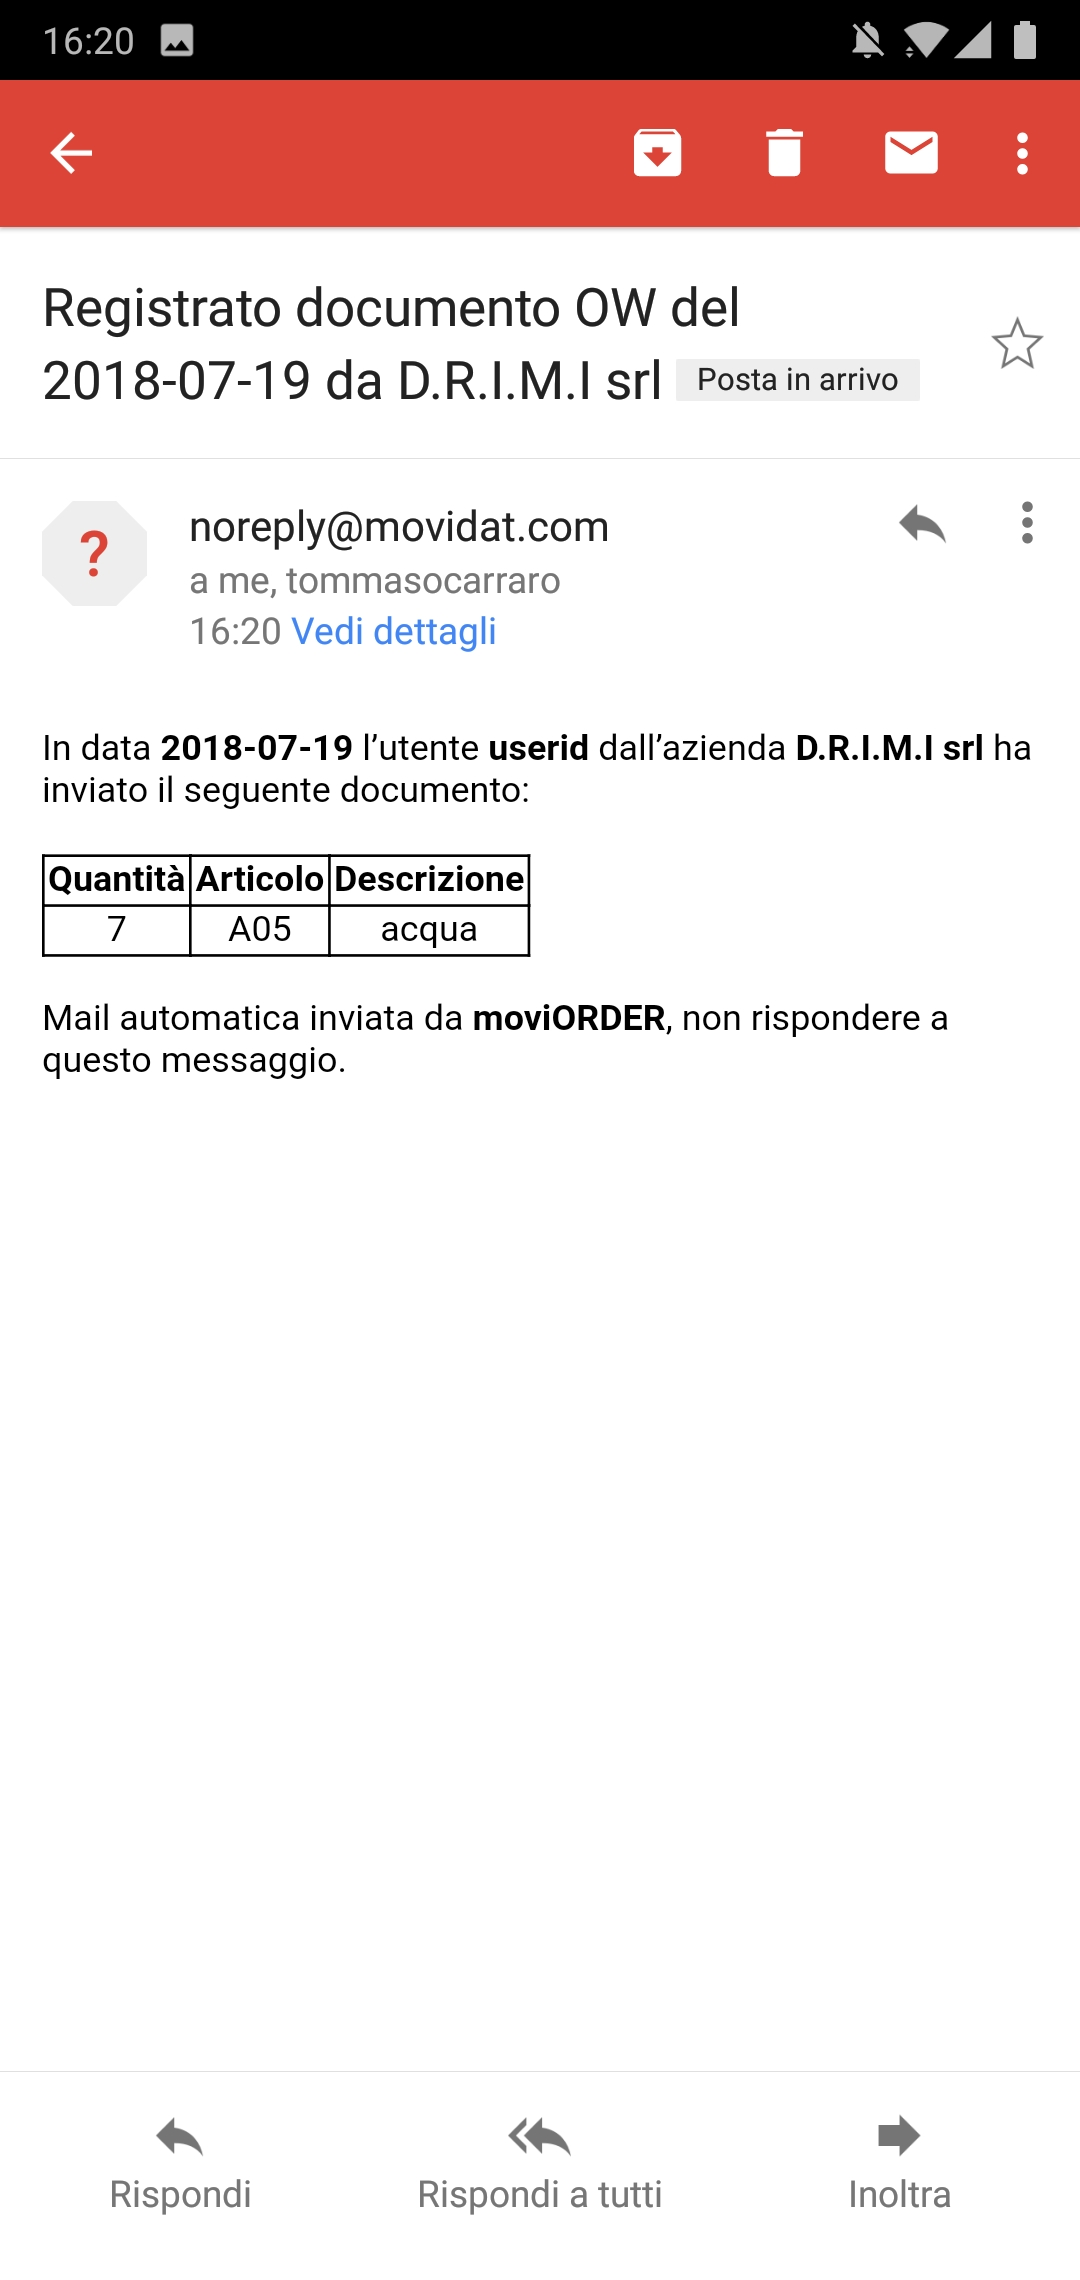
\includegraphics[width=.3\textwidth,height=9cm]{./img/templatemail.jpg}
	\caption{Mail di notifica di un ordine}
\end{figure}